\documentclass[conference,letterpaper]{IEEEtran}
\usepackage{tikz}
\usetikzlibrary{decorations.pathreplacing}
\usepackage[utf8]{inputenc}
\usepackage[T1]{fontenc}
\usepackage[cmex10]{amsmath}

\begin{document}

    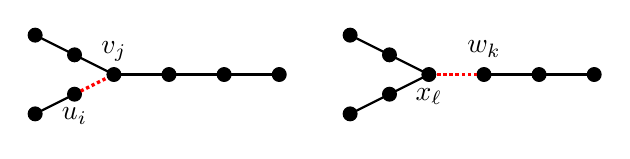
\begin{tikzpicture}[scale=1]

    \tikzstyle{every node}=[draw,circle,fill=black,minimum size=5pt, inner sep=0pt, outer sep=0pt]

    \draw (0,0.5) node (b1) {};
    \draw (0.5,0.75) node (b2) [label=below:$u_i$]{};
    \draw (1,1) node (b3) [label=above:$v_j$]{};
    \draw (0.5,1.25) node (b4) {};
    \draw (0,1.5) node (b5) {};
    \draw (1.7,1) node (b6) {};
    \draw (2.4,1) node (b7) {};
    \draw (3.1,1) node (b8) {};
    \draw[thick, black] (b1) to (b2);
    \draw[thick, black] (b5) to (b3);
    \draw[thick, black] (b3) to (b8);

    \draw[very thick, red, densely dotted] (b2) to (b3);

    \draw (4,0.5) node (c1) {};
    \draw (4.5,0.75) node (c2) {};
    \draw (5,1) node (c3) [label=below:$x_\ell$]{};
    \draw (4.5,1.25) node (c4) {};
    \draw (4,1.5) node (c5) {};
    \draw (5.7,1) node (c6) [label=above:$w_k$]{};
    \draw (6.4,1) node (c7) {};
    \draw (7.1,1) node (c8) {};
    \draw[thick, black] (c1) to (c3);
    \draw[thick, black] (c5) to (c3);
    \draw[thick, black] (c6) to (c8);

    \draw[very thick, red, densely dotted] (c6) to (c3);

\end{tikzpicture}

\end{document}